\begin{figure}[H]
	\centering
	\begin{minipage}{0.4\linewidth}
		\centering
		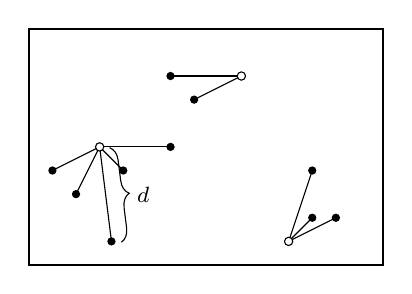
\begin{tikzpicture}[scale=0.3]
		
		\draw [<->,thick] (0,0) rectangle (15,10) {};
		%centroids
		
		%Left Group
%		\fill ( 7,7) circle (5pt);
		\fill ( 1,4) circle (5pt);
		\fill ( 4,4) circle (5pt);
		\fill ( 2,3) circle (5pt);
		\fill (3.5,1) circle (5pt);
		\fill ( 6,5) circle (5pt);
		
		%Middle Group
		
		\fill ( 7,7) circle (5pt);
		\fill ( 6,8) circle (5pt);
		
		%Right Group
		\fill (12,2) circle (5pt);
		\fill (12,4) circle (5pt);
		\fill (13,2) circle (5pt);
		
		%Lines
		\draw [-] (1,4) -- (3,5);
		\draw [-] (4,4) -- (3,5);
		\draw [-] (2,3) -- (3,5);
		\draw [-] (3.5,1) -- (3,5);
		\draw [-] (6,5) -- (3,5);
		
		\draw [-] (7,7) -- (9,8);
		\draw [-] (6,8) -- (9,8);
		
		\draw [-] (12,2) -- (11,1);
		\draw [-] (12,4) -- (11,1);
		\draw [-] (13,2) -- (11,1);
		\fill [white] (11,1) circle (5pt);
		\fill [white] ( 3,5) circle (5pt);
		\fill [white] ( 9,8) circle (5pt);
		
		\draw (11,1) circle (5pt);
		\draw ( 3,5) circle (5pt);
		\draw ( 9,8) circle (5pt);
		
		\draw [decorate,decoration={brace,amplitude=5pt},xshift=12pt,yshift=-1pt]
		(3,5) -- (3.5,1)node [black,midway,xshift=10pt] {\footnotesize$d$};
		\end{tikzpicture}
		\caption*{Non-optimal Assignment}
		\label{fig:badcov}
	\end{minipage}
	\begin{minipage}{0.4\linewidth}
		\centering
		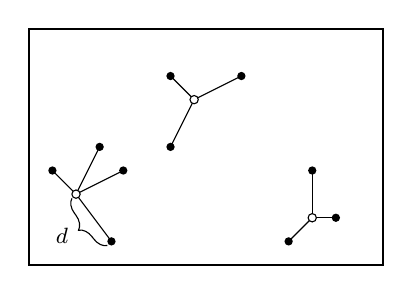
\begin{tikzpicture}[scale=0.3]
		
		\draw [<->,thick] (0,0) rectangle (15,10) {};
		%centroids
		
		%Left Group
		\fill ( 1,4) circle (5pt);
		\fill ( 4,4) circle (5pt);
		\fill ( 3,5) circle (5pt);
		\fill (3.5,1) circle (5pt);
		
		%Middle Group
		\fill ( 6,5) circle (5pt);
		\fill ( 9,8) circle (5pt);
		\fill ( 6,8) circle (5pt);
		
		%Right Group
		\fill (11,1) circle (5pt);
		\fill (12,4) circle (5pt);
		\fill (13,2) circle (5pt);
		
		%\pause
		%Lines
		\draw [-] (1,4) -- (2,3);
		\draw [-] (4,4) -- (2,3);
		\draw [-] (3,5) -- (2,3);
		\draw [-] (3.5,1) -- (2,3);
		
		\draw [-] (6,5) -- (7,7);
		\draw [-] (9,8) -- (7,7);
		\draw [-] (6,8) -- (7,7);
		
		\draw [-] (11,1) -- (12,2);
		\draw [-] (12,4) -- (12,2);
		\draw [-] (13,2) -- (12,2);
		
		\fill [white] ( 2,3) circle (5pt);
		\fill [white] (12,2) circle (5pt);
		\fill [white] ( 7,7) circle (5pt);
		
		\draw ( 2,3) circle (5pt);
		\draw (12,2) circle (5pt);
		\draw ( 7,7) circle (5pt);
		
		%Circles
		%\draw [dashed] (2,3) circle (2.5);
		%\draw [dashed] (7,7) circle (2.236);
		%\draw [dashed] (12,2) circle (2);
		%\pause
		\draw [decorate,decoration={brace,amplitude=5pt},xshift=-5pt,yshift=-5pt]
		(3.5,1) -- (2,3)node [black,midway,xshift=-10pt,yshift=-5pt] {\footnotesize$d$};
		\end{tikzpicture}		
		\caption*{Optimal Assignment}
		\label{fig:goodcov}
	\end{minipage}
	\caption{Different assignments for the same set of points}
	\label{fig:cov}
\end{figure}